\chapter{Sorting}

\section{Introduction}
Why sorting is important

Give an example of sortin
\begin{description}
\item[Stable] When sorting some kinds of data, only part of the data is examined when determining the sort order. For example a deck of card can be orderd by means of the rank ignoring the seed yelding to multiple different valid sorting. A stable sorting algorithm ensure that the order of equal element will be preserved. 
\item[Adaptive]	A sorting algorithm falls into the adaptive sort family if it takes advantage of existing order in its input.  It benefits from the presortedness in the input sequence (or limited disorder) to sort faster. Time complexity is function of input size and entropy.
\item [Online] Online; i.e., can sort a list as it receives it
\end{description}

\section{Bubble-Sort}
Bubble sort, sometimes referred to as sinking sort, is a simple sorting algorithm that repeatedly steps through the list to be sorted, compares each pair of adjacent items and swaps them if they are in the wrong order. The pass through the list is repeated until no swaps are needed, which indicates that the list is sorted. The algorithm, which is a comparison sort, is named for the way smaller elements "bubble" to the top of the list. Although the algorithm is simple, it is too slow and impractical for most problems even when compared to insertion sort (see \ref{sec:insertionsort} at page \pageref{sec:insertionsort}). \textbf{Bubble sort is stable and adaptive}.

The distance and direction that elements must move during the sort determine bubble sort's performance because elements move in different directions at different speeds. An element that must move toward the end of the list can move quickly because it can take part in successive swaps. For example, the largest element in the list will win every swap, so it moves to its sorted position on the first pass even if it starts near the beginning. On the other hand, an element that must move toward the beginning of the list cannot move faster than one step per pass, so elements move toward the beginning very slowly. If the smallest element is at the end of the list, it will take $n-1$ passes to move it to the beginning. This has led to these types of elements being named rabbits and turtles, respectively, after the characters in Aesop's fable of The Tortoise and the Hare.

\begin{lstlisting}[language=C++, caption="Bubble-sort implementation in C++14"]
// CMP_FN has type: D -> D -> bool
template <typename Iterator, typename CMP_FN>
void bubblesort(Iterator s, Iterator e, CMP_FN cmp) {
  auto it1 = s;
  for (; it1 != e; it1++) {
    auto it2 = s;
    for (; it2 != it1; it2++)
      if (cmp(*it1, *it2)) 
      		std::swap(*it1, *it2);
  }
}
\end{lstlisting}

\subsection{Complexity Analysis}
Complexity is $\mathcal{O}(n^2)$ in worst and averge case. Being adaptive it takes advantage of already sorted (or nearly sorted) input. In this case the complexity is $\mathcal{O}(2n)$.
Bubble sort is asymptotically equivalent in running time to insertion sort in the worst case, but the two algorithms differ greatly in the number of swaps necessary. Experimental results such as those of Astrachan have also shown that insertion sort performs considerably better even on random lists. For these reasons many modern algorithm textbooks avoid using the bubble sort algorithm in favor of insertion sort.
Bubble sort also interacts poorly with modern CPU hardware. It requires at least twice as many writes as insertion sort, twice as many cache misses, and asymptotically more branch mispredictions. Experiments by Astrachan sorting strings in Java show bubble sort to be roughly one-fifth as fast as an insertion sort and $70\%$ as fast as a selection sort.
The only significant advantage that bubble sort has over most other implementations, even quicksort, but not insertion sort, is that the ability to detect that the list is sorted efficiently is built into the algorithm. When the list is already sorted (best-case), the complexity of bubble sort is only $\mathcal{O}(2n)$

\section{Insertion-Sort}
\label{sec:insertionsort}
Insertion sort is a simple sorting algorithm that builds the final sorted array (or list) one item at a time. It is much less efficient on large lists than more advanced algorithms such as quicksort, heapsort, or merge sort. However, insertion sort provides several advantages.
It is more efficient in practice than most other simple quadratic (i.e., $\mathcal{O}(n^2)$) algorithms such as selection sort or bubble sort. It is stable and adaptive.Infact when the input is nearly sorted its complexity becomes $\mathcal{O}(nk)$ (when each element is no more than k places away from its sorted position). Can also be easily implemented in-place (using $\mathcal{O}(1)$ additional memory).

It works keeping the first part of the data sorted and iterating on the rest of the data. For each element not already sorted the method finds its sorted position in the first part (the already sorted) of the data.

Sorting is typically done in-place, by iterating up the array, growing the sorted list behind it. At each array-position, it checks the value there against the largest value in the sorted list (which happens to be next to it, in the previous array-position checked). If larger, it leaves the element in place and moves to the next. If smaller, it finds the correct position within the sorted list, shifts all the larger values up to make a space, and inserts into that correct position.
The resulting array after k iterations has the property where the first k + 1 entries are sorted ("+1" because the first entry is skipped). In each iteration the first remaining entry of the input is removed, and inserted into the result at the correct position, thus extending the result:

\begin{figure}
		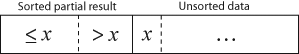
\includegraphics[width=8cm]{Insertionsort-before.png}
\end{figure}

\begin{figure}
		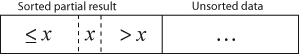
\includegraphics[width=8cm]{Insertionsort-after.png}
	\end{figure}


\begin{lstlisting}[language=c++, caption="Bubble-sort implementation in C++14"]
// CMP_FN has type: D -> D -> bool
template < typename Container, typename CMP_FN>
void insertionsort(Container& v, const int s,const int e, CMP_FN cmp) {
    for(int i=s+1 ; i<e; i++){
        int el = v[i];
        int j = i-1;
        while(cmp(el,v[j]) && j>=s){
            v[j+1] = v[j];
            j--;
        }
        v[j+1]=el;
    }
}
\end{lstlisting}

Suppose we have an array A, and that the subarray from index 0 through index $k$ is already sorted, and we want to insert the element currently in index $k+1$ into this sorted subarray, so that the subarray from index 0 through index $k+1$ is sorted. 
To insert the element in position $k+1$ into the subarray to its left, we repeatedly compare it with elements to its left , going right to left. Let's call the element in position $k+1$ the key. Each time we find that the key is less than an element to its left, we slide that element one position to the right, since we know that the key will have to go to that element's left. We'll need to do two things to make this idea work: we need to have a slide operation that slides an element one position to the right, and we need to save the value of the key in a separate place (so that it doesn't get overridden by the element to its immediate left). 

Here an Haskell implementation of \textit{insertion sort}
\begin{lstlisting}[language=Haskell,caption="Haskell Insertion sort "]
 insert :: Ord a => a -> [a] -> [a]
 insert item []  = [item]
 insert item (h:t) | item <= h = item:h:t
                   | otherwise = h:(insert item t)

 insertsort :: Ord a => [a] -> [a]
 insertsort []    = []   
 insertsort (h:t) = insert h (insertsort t)
\end{lstlisting}

\subsection{Complexity Analysis}
Time complexity is  $\mathcal{O}(n^2)$ while spatial complexity is  $\mathcal{O}(1)$. It is adaptive, and when each element does not move more than $k$ position from the original position to the sorted location its complexity is linear:  $\mathcal{O}(nk)$.   As for bubble-sort its best case is linear, but it performs much less operations mainly because bubble-sort is a \textit{exchange} algorithm while insertion sort is a \textit{shifting} one. Exchange requires a third of the operation of \textit{shifting}.

\section{Selection-Sort}
Selection sorting is conceptually the most simplest sorting algorithm. This algorithm first finds the smallest element in the array and exchanges it with the element in the first position, then find the second smallest element and exchange it with the element in the second position, and continues in this way until the entire array is sorted. 

The algorithm divides the input list into two parts: the sublist of items already sorted, which is built up from left to right at the front (left) of the list, and the sublist of items remaining to be sorted that occupy the rest of the list. Initially, the sorted sublist is empty and the unsorted sublist is the entire input list. The algorithm proceeds by finding the smallest (or largest, depending on sorting order) element in the unsorted sublist, exchanging (swapping) it with the leftmost unsorted element (putting it in sorted order), and moving the sublist boundaries one element to the right.

\begin{verbatim}
64 25 12 22 11 // this is the initial, starting state of the array

11 25 12 22 64 // sorted sublist = {11}

11 12 25 22 64 // sorted sublist = {11, 12}

11 12 22 25 64 // sorted sublist = {11, 12, 22}

11 12 22 25 64 // sorted sublist = {11, 12, 22, 25}

11 12 22 25 64 // sorted sublist = {11, 12, 22, 25, 64}
\end{verbatim}
\subsection{Complexity Analysis}
Time complexity is  $\mathcal{O}(n^2)$ and is generally slower than insertion sort and is not used in production code except when memory is very limited.





\section{Merge-Sort}
In computer science, merge sort (also commonly spelled mergesort) is an efficient, general-purpose, comparison-based sorting algorithm. Most implementations produce a stable sort, which means that the implementation preserves the input order of equal elements in the sorted output. Mergesort is a divide and conquer algorithm that was invented by John von Neumann in 1945.

Conceptually, a merge sort works as follows:
\begin{enumerate}
\item Divide the unsorted list into n sublists, each containing 1 element (a list of 1 element is considered sorted).
\item Repeatedly merge sublists to produce new sorted sublists until there is only 1 sublist remaining. This will be the sorted list.
\end{enumerate} 

Merge is the most important part of the algorithm. Merge algorithms are a family of algorithms that take multiple sorted lists as input and produce a single list as output, containing all the elements of the inputs lists in sorted order. These algorithms are used as subroutines in various sorting algorithms, most famously merge sort.

In particular merging two sorted collections into one can be done in linear time and linear space.When the inputs are linked lists, this algorithm can be implemented to use only a constant amount of working space; the pointers in the lists' nodes can be reused for bookkeeping and for constructing the final merged list.

\begin{lstlisting}[language=c++, caption="Bubble-sort implementation in C++14"]
// CMP_FN has type: D -> D -> bool
//[s1,e1] and [e1+1,e2] are two ordered sequences. This methods reaggarne the whole
// interval [s1,e2] in a sorted sequence
template < typename Container, typename CMP_FN>
void merge(Container& v, Container& scratch,  int s1,  int e1,  int e2,CMP_FN cmp){
    int s2 = e1+1;
    int ins =0;
    int b = s1;
    while(s1 <= e1 && s2<=e2)
        if(cmp(v[s1],v[s2]))
            scratch[b+ins++] = v[s1++];
        else
            scratch[b+ins++] = v[s2++];
    while(s1 <= e1)
        scratch[b+ins++] = v[s1++];
    while(s2 <= e2)
        scratch[b+ins++] = v[s2++];
        
    for(int i=0 ; i < ins ; i++)
        v[b+i] = scratch[b+i];
}
\end{lstlisting}

The following is the main mergesort method. It uses an helper function in order to hide the additional space required by the merge. Note that midpoint is computed using the \texttt{safe\_midpoint()} methods which avoids overflows for large $lo$ and $hi$ at a cost of an additional operation.

\begin{lstlisting}[language=c++, caption="Merge-sort"]
template<typename T>
inline T safe_midpoint(const T lo, const T hi){
    return lo+(hi-lo)/2;
}
template<typename T>
inline T unsafe_midpoint(const T lo, const T hi){
    return (hi+lo)/2;
}
#define TRIGGER_INSERTIONSORT (4)
template < typename Container, typename CMP_FN>
void mergesort_helper(Container& v,Container& scratch, const int s,const int e, CMP_FN cmp) {
    if(e -s <= TRIGGER_INSERTIONSORT)
        DS::insertionsort(v,s,e,cmp);
    if(s < e){
        int midpoint = safe_midpoint(s,e);
        mergesort_helper(v,scratch,s,midpoint,cmp);
        mergesort_helper(v,scratch,midpoint+1,e,cmp);
        merge(v,scratch,s,midpoint,e,cmp);
    }
}
// CMP_FN has type: D -> D -> bool
template < typename Container, typename CMP_FN>
void mergesort(Container& v, const int s,const int e, CMP_FN cmp) {
    Container scratch(v.size());
    mergesort_helper(v,scratch,s,e,cmp);

}
\end{lstlisting}


\textbf{QuickSort is better for contiguous data structures}.
In the merge sort algorithm, this subroutine is typically used to merge two sub-arrays $A[lo..mid]$, $A[mid..hi]$ of a single array $A$. This can be done by copying the sub-arrays into a temporary array, then applying the merge algorithm above.The allocation of a temporary array can be avoided, but at the expense of speed and programming ease. Various in-place merge algorithms have been devised, sometimes sacrificing the linear-time bound to produce an $\mathcal{nlog(n)}(n^2)$ algorithm.

Quick Sort in its general form is an in-place sort (i.e. it does not require any extra storage) whereas merge sort requires $O(N)$ extra storage, where $N$ denote the array size which may be quite expensive. Allocating and de-allocating the extra space used for merge sort increases the running time of the algorithm. Comparing average complexity we find that both type of sorts have $O(NlogN)$ average complexity but the constants differ (and sometimes matter). For arrays, merge sort loses due to the use of extra $O(N)$ storage space.

Most practical implementations of Quick Sort use randomized version. The randomized version has expected time complexity of O(nLogn). The worst case is possible in randomized version also, but worst case doesn’t occur for a particular pattern (like sorted array) and randomized Quick Sort works well in practice.
Quick Sort is also a cache friendly sorting algorithm as it has good locality of reference when used for arrays.
Quick Sort is also tail recursive, therefore tail call optimizations is done.

\textbf{Merge-Sort is better for Linked Data Structure}.
List case is different mainly due to differenc in memory allocation patterns w.t.r. to array.In linked list, we can insert items in the middle in $O(1)$ extra space and time. Therefore merge operation of merge sort can be implemented without extra space for linked lists (i.e. no waste of time during allocation and copy of any extra buffers). 
For contiguous data structure, we can do $O(1)$ time and space random access as elements are continuous in memory. But  Unlike arrays, we can not do random access in linked list \footnote{In linked list to access $i^{th}$ element, we have to travel each and every node from the head to $i^{th}$ node as we don not have continuous block of memory}. Quick Sort requires a lot of this kind of accesses. Therefore, the overhead increases for quick sort. Merge sort accesses data sequentially and the need of random access is low.


\subsubsection{Iterative Merge-Sort}

\subsection{Complexity Analysis}

Merge Sort is a recursive algorithm and time complexity can be expressed as following recurrence relation.
$T(n) = 2T(n/2) + \Theta(n)$
The above recurrence can be solved either using Recurrence Tree method or Master method. It falls in case II of Master Method and solution of the recurrence is $\Theta(nlog(n))$.
Time complexity of Merge Sort is $\Theta(nlog(n))$ in all 3 cases (worst, average and best) as merge sort always divides the array in two halves and take linear time to merge two halves.
Auxiliary Space: $O(n)$
Sorting In Place: No in a typical implementation
Stable: Yes




\section{Quick-Sort}

\subsection{Complexity Analysis}

\section{Heap-Sort}

\subsection{Complexity Analysis}

\section{Smoot-Sort}

\subsection{Complexity Analysis}


\section{Solving Recurrence relation}

\section{Substitution method}
\label{sec:substitutionmethod}
Despite the name, this is not a method that gives us a solution for the recurrence. It serves only to prove that an initial solution guess is right. It basically use induction to prove that the guess holds and is an actual solution of the recurrence equation.


\section{Recursion Tree method}
A recursion tree is useful for visualizing what happens when a recurrence is iterated. It diagrams the tree of recursive calls and the amount of work done at each call.
For instance, consider the recurrence
\[T(n) = 2T(\frac{n}{2}) + n^2\]
The recursion tree for this recurrence has the following form(see figure \ref{fig:rectree1})

\begin{figure}
\label{fig:rectree1}
		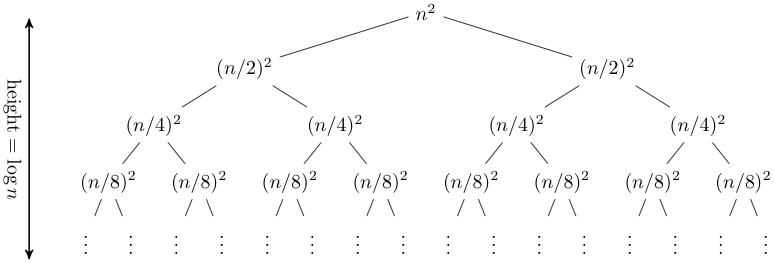
\includegraphics[width=12cm]{recTree1.png}
\end{figure}
It is easy to compute the amount of work done at each recursion level simply summing up all the nodes at a certain level (see figure \ref{fig:rectree2}).
\begin{figure}
\label{fig:rectree2}
		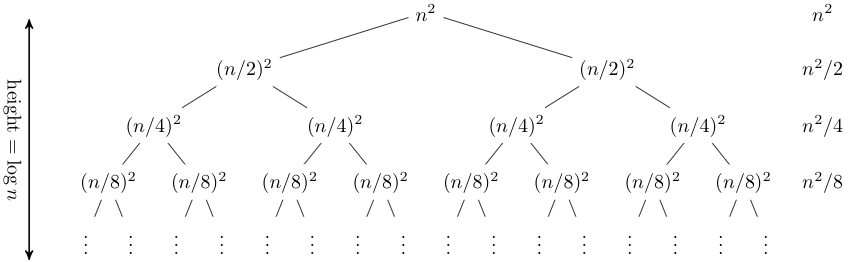
\includegraphics[width=12cm]{recTree2.png}
\end{figure}

In this case this is a geometric serie which sum limit is bounded by a quadratic function i.e. $O(n^2)$. 

Recursion trees can be useful for gaining intuition about the closed form of a recurrence, but they are not a proof (and in fact it is easy to get the wrong answer with a recursion tree, as is the case with any method that includes ''...'' kinds of reasoning). As we saw last time, a good way of establishing a closed form for a recurrence is to make an educated guess and then prove by induction that your guess is indeed a solution (see section \ref{sec:substitutionmethod} at page \ref{sec:substitutionmethod}). Recurrence trees can be a good method of guessing.


For example consider the following recurrence equation:
\[ T(n) = T(\frac{n}{3}) + T(\frac{2n}{3}) + n\]

Expanding the first levels of the corrensponding recursion tree we obtain the tree in figure \ref{fig:rectree3}.
\begin{figure}
\label{fig:rectree3}
		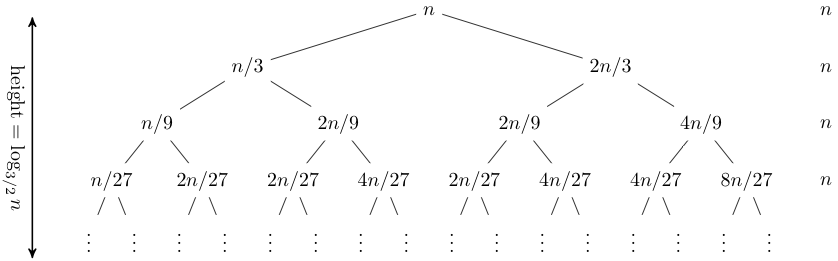
\includegraphics[width=12cm]{recTree3.png}
\end{figure}

Each level sums up to $n$, the height of this tree is $log_{\frac{3}{2}}(n)$. So out guess is that $T=O(nlogn)$.

Using the substitution method let's check if our guess is right.

\section{Master method}




\section{Questions \& Problems}
%---Question ------------
\begin{problem}
Which of the following is not a stable sorting algorithm in its typical implementation.
\begin{enumerate}
\item Insertion-sort
\item Merge-sort
\item Quick-sort
\item Bubble-sort
\end{enumerate}

\end{problem}

%---Question------------
\begin{problem}
Consider a situation where swap operation is very costly. Which of the following sorting algorithms should be preferred so that the number of swap operations are minimized in general?
\begin{enumerate}
\item Insertion-sort
\item Merge-sort
\item Quick-sort
\item Bubble-sort
\end{enumerate}

\end{problem}



%---Question------------
\begin{problem}
You have to sort 1 GB of data with only 100 MB of available main memory. Which sorting technique will be most appropriate?
\begin{enumerate}
\item Insertion-sort
\item Merge-sort
\item Quick-sort
\item Bubble-sort
\end{enumerate}

\end{problem}


%---Question------------
\begin{problem}
In a modified merge sort, the input array is splitted at a position one-third of the length(N) of the array. What is the worst case time complexity of this merge sort?
\begin{enumerate}
\item $\mathcal{O}(nlog_3(n))$
\item $\mathcal{O}(nlog_{\frac{2}{3}}(n))$
\item $\mathcal{O}(nlog_{\frac{1}{3}}(n))$
\item $\mathcal{O}(nlog_{\frac{3}{2}}(n))$

\end{enumerate}

\end{problem}


%---Question------------
\begin{problem}
Which sorting algorithm will take least time when all elements of input array are identical? Consider typical implementations of sorting algorithms.
\begin{enumerate}
\item Insertion-sort
\item Merge-sort
\item Quick-sort
\item Bubble-sort
\end{enumerate}

\end{problem}


%---Question------------
\begin{problem}
A list of n string, each of length n, is sorted into lexicographic order using the merge-sort algorithm. The worst case running time of this computation is:
\begin{enumerate}
\item $\mathcal{O}(nlog(n))$
\item $\mathcal{O}(n^2log(n))$
\item $\mathcal{O}(n^2 + log(n))$
\item $\mathcal{O}(n^2)$
\end{enumerate}

\end{problem}


%---Question1------------
\begin{problem}
Which of the following sorting algorithms has the lowest worst-case complexity?
\begin{enumerate}
\item Insertion-sort
\item Merge-sort
\item Quick-sort
\item Bubble-sort
\end{enumerate}

\end{problem}



%---Question1------------
\begin{problem}
Which of the following is true about merge sort?
\begin{enumerate}
\item Merge Sort works better than quick sort if data is accessed from slow sequential memory.
\item Merge Sort is stable sort by nature
\item Merge sort outperforms heap sort in most of the practical situations.
\item All the above.
\end{enumerate}

\end{problem}


%---Question1------------
\begin{problem}
Assume that a mergesort algorithm in the worst case takes 30 seconds for an input of size 64. Which of the following most closely approximates the maximum input size of a problem that can be solved in 6 minutes?
\begin{enumerate}
\item $2^8$
\item $2^9$
\item $2^{10}$
\item $2^{11}$
\end{enumerate}

\end{problem}



%---Problem------------
\begin{problem}
\textit{Given an array, write a program that prints 1 if array is sorted in non-decreasing order, else prints 0.}

\textbf{Input:}
The first line of input contains an integer $T$ denoting the number of test cases.
The first line of each test case contains $N$, which is the size of array (on the following line).
The second line of each test case contains $N$ input $C[i]$.

\textbf{Output:}
Print 1 if array is sorted, else print 0.

\textbf{Constraints:}
\begin{multline}\\
1 \leq T \leq 100\\
1 \leq N \leq 500\\
1 \leq C[i] \leq 1200\\
\end{multline}
\end{problem}

\begin{solution}
\begin{lstlisting}[language=C++, caption="C++ Solution"]
	int main(){
		return 0;	
	}
\end{lstlisting}

\end{solution}



%---Problem------------
\begin{problem}
\textit{Given a binary array, sort it in non-decreasing order.}

\textbf{Input:}
First line contains an integer denoting the test cases $T$.  Every test case contains two lines, first line is size $N$ and second line is space separated elements of array

\textbf{Output:}
Space separated elements of sorted arrays.  There should be a new line between output of every test case.

\textbf{Constraints:}
\begin{multline}\\
10 \leq T \leq 100\\
1 \leq N \leq 10000\\
\end{multline}

\textbf{Example:}
\begin{verbatim}
Input:
2
5
1 0 1 1 0
10
1 0 1 1 1 1 1 0 0 0

Output:
0 0 1 1 1
0 0 0 0 1 1 1 1 1 1 

\end{verbatim}

\end{problem}

\begin{solution}
\begin{lstlisting}[language=C++, caption="C++ Solution"]
	int main(){
		return 0;	
	}
\end{lstlisting}

\end{solution}



%---Problem------------
\begin{problem}
\textit{Given an array, print k largest elements from the array.}

\textbf{Input:}
The first line of input contains an integer $T$ denoting the number of test cases.
The first line of each test case is $N$ and $K$, where $N$ is the size of array and $K$ is the largest elements to be returned.
The second line of each test case contains $N$ input $C[i]$.

\textbf{Output:}
Print the $K$ largest elements in \textbf{descending order}.

\textbf{Constraints:}
\begin{multline}\\
10 \leq T \leq 50\\
1 \leq N \leq 100\\
K \leq N \\
1 \leq C[i] \leq 1000\\
\end{multline}

\textbf{Example:}
\begin{verbatim}
Input:
2
5 2
12 5 787 1 23
7 3
1 23 12 9 30 2 50

Output:
787 23
50 30 23

\end{verbatim}

\end{problem}

\begin{solution}
\begin{lstlisting}[language=C++, caption="C++ Solution"]
	int main(){
		return 0;	
	}
\end{lstlisting}

\end{solution}



%---Problem------------
\begin{problem}
Given an array with n distinct elements, convert the given array to a reduced form where all elements are in range from $[0 ... n-1]$. The order of elements is same, i.e., 0 is placed in place of smallest element, 1 is placed for second smallest element,\ldots $n-1$ is placed as last element.

\textbf{Input:}
The first line of input contains an integer $T$ denoting the number of test cases.
The first line of each test case is $N$, where $N$ is the size of array.
The second line of each test case contains $N$ input $A[i]$.

\textbf{Output:}
Print the reduced form of the array.

\textbf{Constraints:}
\begin{multline}\\
1 \leq T \leq 100\\
1 \leq N \leq 200\\
1 \leq A[i] \leq 500\\
\end{multline}

\textbf{Example:}
\begin{verbatim}
Input:
2
3
10 40 20
5
5 10 40 30 20

Output:
0 2 1
0 1 4 3 2

\end{verbatim}

\end{problem}


%---Problem------------
\begin{problem}
Given two array $A1$ and $A2$, sort $A1$ in such a way that the relative order among the elements will be same as those are in $A2$. For the elements not present in $A2$. Append them at last in sorted order.

\textbf{Input:}
The first line of input contains an integer $T$ denoting the number of test cases.
The first line of each test case is $M$ and $N,M$ are the number of elements in $A1$ and $A2$ respectively.
The second line of each test case contains $M$ elements.
The third line of each test case contains $N$ elements.
\textbf{Output:}
Print the sorted array according order defined by another array.

\textbf{Constraints:}
\begin{multline}\\
1 \leq T \leq 50\\
1 \leq N \leq M \leq 10\\
1 \leq A1[i],A2[i] \leq 500\\
\end{multline}

\textbf{Example:}
\begin{verbatim}
Input:
2
3
10 40 20
5
5 10 40 30 20

Output:
0 2 1
0 1 4 3 2

\end{verbatim}

\end{problem}


\begin{solution}
\begin{lstlisting}[language=C++, caption="C++ Solution"]
	int main(){
		return 0;	
	}
\end{lstlisting}

\end{solution}


%---Problem------------
\begin{problem}
\textit{Given an array of integers, sort the array according to frequency of elements. For example, if the input array is $\{2, 3, 2, 4, 5, 12, 2, 3, 3, 3, 12\}$, then modify the array to $\{3, 3, 3, 3, 2, 2, 2, 12, 12, 4, 5\}$}. 

If frequencies of two elements are same, print them in increasing order.

\textbf{Input:}
The first line of input contains an integer $T$ denoting the number of test cases. The description of $T$ test cases follows. The first line of each test case contains a single integer $N$ denoting the size of array. The second line contains $N$ space-separated integers $A1, A2, ..., AN$ denoting the elements of the array.

\textbf{Output:}
Print each sorted array on a newline. Each sorted array should be printed as space-separated.

\textbf{Constraints:}
\begin{multline}\\
1 \leq T \leq 70\\
1 \leq N \leq 130\\
1 \leq A[i] \leq 60\\
\end{multline}

\textbf{Example:}
\begin{verbatim}
Input:
1
5
5 5 4 6 4

Output:
4 4 5 5 6 

\end{verbatim}

\end{problem}

\begin{solution}
\begin{lstlisting}[language=C++, caption="C++ Solution"]
	int main(){
		return 0;	
	}
\end{lstlisting}

\end{solution}

